\documentclass{article}[18pt]
\ProvidesPackage{format}
%Page setup
\usepackage[utf8]{inputenc}
\usepackage[margin=0.7in]{geometry}
\usepackage{parselines} 
\usepackage[english]{babel}
\usepackage{fancyhdr}
\usepackage{titlesec}
\hyphenpenalty=10000

\pagestyle{fancy}
\fancyhf{}
\rhead{Sam Robbins}
\rfoot{Page \thepage}

%Characters
\usepackage{amsmath}
\usepackage{amssymb}
\usepackage{gensymb}
\newcommand{\R}{\mathbb{R}}

%Diagrams
\usepackage{pgfplots}
\usepackage{graphicx}
\usepackage{tabularx}
\usepackage{relsize}
\pgfplotsset{width=10cm,compat=1.9}
\usepackage{float}

%Length Setting
\titlespacing\section{0pt}{14pt plus 4pt minus 2pt}{0pt plus 2pt minus 2pt}
\newlength\tindent
\setlength{\tindent}{\parindent}
\setlength{\parindent}{0pt}
\renewcommand{\indent}{\hspace*{\tindent}}

%Programming Font
\usepackage{courier}
\usepackage{listings}
\usepackage{pxfonts}

%Lists
\usepackage{enumerate}
\usepackage{enumitem}

% Networks Macro
\usepackage{tikz}


% Commands for files converted using pandoc
\providecommand{\tightlist}{%
	\setlength{\itemsep}{0pt}\setlength{\parskip}{0pt}}
\usepackage{hyperref}

% Get nice commands for floor and ceil
\usepackage{mathtools}
\DeclarePairedDelimiter{\ceil}{\lceil}{\rceil}
\DeclarePairedDelimiter{\floor}{\lfloor}{\rfloor}

% Allow itemize to go up to 20 levels deep (just change the number if you need more you madman)
\usepackage{enumitem}
\setlistdepth{20}
\renewlist{itemize}{itemize}{20}

% initially, use dots for all levels
\setlist[itemize]{label=$\cdot$}

% customize the first 3 levels
\setlist[itemize,1]{label=\textbullet}
\setlist[itemize,2]{label=--}
\setlist[itemize,3]{label=*}

% Definition and Important Stuff
% Important stuff
\usepackage[framemethod=TikZ]{mdframed}

\newcounter{theo}[section]\setcounter{theo}{0}
\renewcommand{\thetheo}{\arabic{section}.\arabic{theo}}
\newenvironment{important}[1][]{%
	\refstepcounter{theo}%
	\ifstrempty{#1}%
	{\mdfsetup{%
			frametitle={%
				\tikz[baseline=(current bounding box.east),outer sep=0pt]
				\node[anchor=east,rectangle,fill=red!50]
				{\strut Important};}}
	}%
	{\mdfsetup{%
			frametitle={%
				\tikz[baseline=(current bounding box.east),outer sep=0pt]
				\node[anchor=east,rectangle,fill=red!50]
				{\strut Important:~#1};}}%
	}%
	\mdfsetup{innertopmargin=10pt,linecolor=red!50,%
		linewidth=2pt,topline=true,%
		frametitleaboveskip=\dimexpr-\ht\strutbox\relax
	}
	\begin{mdframed}[]\relax%
		\centering
		}{\end{mdframed}}



\newcounter{lem}[section]\setcounter{lem}{0}
\renewcommand{\thelem}{\arabic{section}.\arabic{lem}}
\newenvironment{defin}[1][]{%
	\refstepcounter{lem}%
	\ifstrempty{#1}%
	{\mdfsetup{%
			frametitle={%
				\tikz[baseline=(current bounding box.east),outer sep=0pt]
				\node[anchor=east,rectangle,fill=blue!20]
				{\strut Definition};}}
	}%
	{\mdfsetup{%
			frametitle={%
				\tikz[baseline=(current bounding box.east),outer sep=0pt]
				\node[anchor=east,rectangle,fill=blue!20]
				{\strut Definition:~#1};}}%
	}%
	\mdfsetup{innertopmargin=10pt,linecolor=blue!20,%
		linewidth=2pt,topline=true,%
		frametitleaboveskip=\dimexpr-\ht\strutbox\relax
	}
	\begin{mdframed}[]\relax%
		\centering
		}{\end{mdframed}}
\lhead{ADS}
\lstset{language=C,
	basicstyle=\ttfamily,
	keywordstyle=\bfseries,
	showstringspaces=false,
	morekeywords={if, else, then, print, end, for, do, while},
	tabsize=4,
	mathescape=true,
	numbers=left,
	stepnumber=1,
}
\usepackage{caption}
\DeclareCaptionFont{white}{\color{white}}
\DeclareCaptionFormat{listing}{\colorbox{gray}{\parbox{\textwidth}{#1#2#3}}}
\captionsetup[lstlisting]{format=listing,labelfont=white,textfont=white}





\usepackage{tikz}


\usepackage[trim]{tokenizer} 

\makeatletter

\newcounter{sncolumncounter}
\newcounter{snrowcounter}

\def \nodelabel#1{%
	\setcounter{snrowcounter}{1}
	\foreach \i in {#1}{%
		\draw (\value{sncolumncounter},\value{snrowcounter}) node[anchor=south]{\i};
		\addtocounter{snrowcounter}{1}
	}
	\addtocounter{sncolumncounter}{1}
}

\def \nodeconnection#1{%
	\foreach \i in {#1}{%
		\GetTokens{nodesrc}{nodedest}{\i}
		\draw (\value{sncolumncounter},\nodesrc) node[circle,fill=black]{}--(\value{sncolumncounter},\nodedest) node[circle,fill=black]{};
	}
	\addtocounter{sncolumncounter}{1}
}

\newenvironment{sortingnetwork}[3]
{
	\setcounter{sncolumncounter}{0}
	\def \sn@fullsize{15}
	\begin{tikzpicture}[scale=#3*\sn@fullsize/#2]
	\foreach \i in {1, ..., #1}
	{
		\draw (0,\i)--(#2-1,\i);
	}
}
{
	\end{tikzpicture}
}
\makeatother



\begin{document}
\begin{center}
\underline{\huge Part 3}
\end{center}
\section{Sorting}
\begin{center}
\textit{For any comparison based sorting algorithm $\mathcal{A}$ and any $n\in \mathbb{N}$ large enough there exists an input of length n that requires $\mathcal{A}$ to perform $\Omega(n\log n)$ comparisons}
\end{center}
\subsection{Bucket Sort}
\begin{lstlisting}[caption={BucketSort($a_1,...,a_n\in \{0,\ldots K-1\},n\geqslant 2$)}]
create array C[0,...,K-1] and initialise each entry C[i] to zero
for i=1 to n do
	increment value C[$a_i$] by one
end for
for i=0 to K-1 do
	for j-1 to C[i] do
		print i
	end for
end for
\end{lstlisting}
\begin{itemize}
	\item This puts elements with key i into the ith bucket, then empties one bucket after another.
	\item Its running time is $\mathcal{O}(n+k)$
	\item This means that if K is small then the running time is $o(n\log n)$, apparently beating our lower bound.
	\item The reason for this is that bucket sort doesn't do any comparisons
	\item Also as K gets really large it becomes the worst sorting algorithm we've seen
\end{itemize}
\subsection{Radix Sort}
\begin{itemize}
	\item With bucket sort if the range of our items is large, then we need a large number of buckets.
	\item An improvement is to not look at item values but "one level below"
\end{itemize}
The idea of radix sort:
\begin{itemize}
	\item Have as many buckets as you've got different digits, so for base 10, 10 buckets
	\item Repeatedly bucket sort by given digit
	\item The number of rounds will depend on values, but number of buckets depends only on number of different digits
\end{itemize}
Radix sort has running time $\Theta(d\cdot n)$ where d is the number of rounds\\
In comparison to bucket sort in range $\{0,...,K-1\}$
\begin{itemize}
	\item Radix sort $d=\log_{10}K$, giving $\Theta(n\cdot \log K)$
	\item Bucket sort $\Theta(n+K)$
\end{itemize}
\section{Searching and Selecting}
Suppose:
\begin{itemize}
	\item You are given an array of n numbers
	\item The numbers are in sorted order
	\item The n numbers are pairwise distinct
	\item The number to be searched for is one of the numbers in the array 
\end{itemize}
\begin{lstlisting}[caption=int trivial\_search ({int A[1...n], int x})]
p=1
while (A[p] != x) do
	p=p+1
end while
return p
\end{lstlisting}
\subsection{Binary Search}
Same assumptions as before
\begin{enumerate}
	\item Peek right into the middle of the given array, at position $p=\lceil n/2 \rceil$
	\item If $A[p]=x$ then we're lucky and done and can return p
	\item Otherwise, if x is greater than A[p], we may focus our search on the elements to the right of A[p] and completely ignore anything to its left. Vice versa with if x is less than A[p]
	\item Then recursively call this function on the smaller list until we find the element
\end{enumerate}
\begin{lstlisting}[caption=int search ({int A[1..n], int left, int right, int x})]
if (right == left and A[left] != x)
	handle error; leave function
p = middle-index between left and right
if (A[p] == x) then
return p
// here come the recursive calls (if x not yet found)
if (x > A[p]) then
	return search(A,p+1,right,x) // in right half
else // x < A[p]
	return search(A,left,p-1,x) // in left half
\end{lstlisting}
The initial call would be \texttt{search(A,1,n,x)}\\
\\
For binary search we have the recurrence
\[
T(n)=T(n / 2)+O(1)=O(\log n)
\]
for large n, which is an awful lot quicker
\subsection{Selection}
So far, we had assumed that
\begin{itemize}
	\item The input is sorted
	\item We are looking for the position p of an element of given value x
\end{itemize}
Now we're changing the setup
\begin{itemize}
	\item Input is unsorted
	\item We're looking for value of the ith smallest element in the input
\end{itemize}
A solution to this is to sort the input in time $\mathcal{O}(n\log n)$ and return the ith element from the left
\subsection{QuickSelect}
This has much the same idea as QuickSort
\begin{itemize}
	\item Recursive
	\item \texttt{Partition()} function for selecting pivot and partitioning into LOW and HIGH
	\item not two recursive calls to sort but now only one: dividing into the part (LOW or HIGH) where we know the ith smallest element is to be found
\end{itemize}
\begin{lstlisting}[caption=QuickSelect ({int A[1..n], int left, int right, int i})]
if (left == right) then
	return A[left]
else
	// rearrange/partition in place
	// return value "pivot" is index of pivot element
	// in A[] after partitioning
	pivot = Partition (A, left, right)
	// Now:
	// everything in A[left...pivot-1] is smaller than pivot
	// everything in A[pivot+1...right] is bigger than pivot
	// the pivot is in correct position w.r.t. sortedness
	if (i == pivot) then
		return A[i]
	else if (i < pivot) then
		return QuickSelect (A, left, pivot-1, i)
	else // i > pivot
		return QuickSelect (A, pivot+1, right, i)
	end if
end if
\end{lstlisting}
In the worst case this will be just as slow as worst case QuickSort
$$T(n)=T(n-1)+\mathcal{O}(n) \ \text{which means} \ T(n)=\Theta(n^2)$$
However choosing the pivot at random makes it $\mathcal{O}(n)$, this is just expectation though, and won't be true all the time
\subsection{Median-of-Medians}
This has a guaranteed linear time complexity
\begin{enumerate}
	\item If length(A)$\leqslant$5, then sort and return the ith smallest
	\item Divide n elements into $\lfloor n/5 \rfloor$ groups of 5 elements each, plus at most one group containing the remaining $n\mod5$ elements
	\item Find the median of each of the $\lceil n/5\rceil$ groups by sorting each one, and then picking median from sorted group elements
	\item Call \textbf{select} recursively on set of $\lceil n/5\rceil$ medians found above, giving median-of-medians, x
	\item Partition the entire input around x. Let k be the number of elements on low side plus one
	\begin{itemize}
		\item x is the kth smallest element, and
		\item there are n-k elements on high side of the partition
	\end{itemize}
	\item if i=k, return x. Otherwise use Select recursively to find ith smallest element of low side if $i<k$, or (i-k)th smallest on high side if $i>k$
\end{enumerate}
\section{Trees}
\textbf{Tree} - A connected graph without cycles\\
\\
Trees can be used to store data in a similar manner to a linked list, so each node has:
\begin{itemize}
	\item Pointer to parent (or NIL, or to itself, if root)
	\item Pointer to left child (or NIL, or to itself, if there isn't one)
	\item Pointer to right child (or NIL, or to itself, if there isn't one)
	\item Payload
\end{itemize}
Trees are good as they have fast insert, lookup and delete operations
\subsection{Binary Search Tree}
\textbf{Binary Search Tree} - A tree in which no node has more than two children\\
\\
The one crucial property of a BST is that you must build and maintain the tree such that it's true for every node v of the tree that:
\begin{itemize}
	\item All elements in its left sub-tree are "smaller" than v
	\item All elements in its right sub-tree are "bigger" than v
\end{itemize}
Different ways to do tree traversals:
\begin{itemize}
	\item In order
	\begin{itemize}
		\item Recurse into left sub-tree, print payload, recurse into right sub-tree	
	\end{itemize}
	\item Pre-order
	\begin{itemize}
		\item Print payload, recurse into sub-trees
	\end{itemize}
	\item Post-order
	\begin{itemize}
		\item Recurse into sub-trees, print payload 			
	\end{itemize}
\end{itemize}
\subsection{RedBlack trees}
All simple BST operations take $\mathcal{O}(h)$ time, where h is the height of the BST
\begin{itemize}
	\item This is OK if the BST is balanced, when $h=\mathcal{O}(\log n)$
	\item This is Bad if the BST is degenerated, then $h=\Omega(n)$
\end{itemize}
A BST is a red-black tree if:
\begin{itemize}
	\item Every node is either red or black
	\item The root is black
	\item Every leaf (\texttt{NULL}) is black
	\item Red nodes have black children
	\item For all nodes, all paths from node to descendant leaves contain the same number of black nodes
\end{itemize}
\begin{center}
\textit{A red-black tree with n internal nodes has height at most 2log(n+1)}
\end{center}
To maintain the red-black property the main building block is rotations
\begin{center}
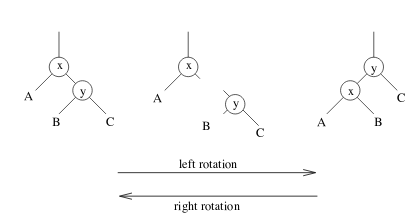
\includegraphics[scale=0.7]{Rotation}
\end{center}
This can be done in $\mathcal{O}(\log n)$\\
\\
A red-black tree has worst case complexities:
\begin{itemize}
	\item space $\mathcal{O}(n)$
	\item lookup $\mathcal{O}(\log n)$
	\item insert $\mathcal{O}(\log n)$
	\item delete $\mathcal{O}(\log n)$
\end{itemize}
\subsection{Heaps}
Heaps are trees, but typically assumed to be stored in a flat array
\begin{itemize}
	\item Each tree node corresponds to an element of the array
	\item The tree is complete except perhaps the lowest level, filled left-to-right
	\item Heap property: for all nodes v in the tree \texttt{v.parent.data>= v.data} (assuming we have a node class like for BSTs)
	\item This is a max-heap (for min-heaps \texttt{v.parent.data =< v.data})
\end{itemize}
Heap represented as an array A has two attributes
\begin{itemize}
	\item \texttt{Length(A)} - the size of the array
	\item \texttt{HeapSize(A)} - the size of the heap stored within the array
\end{itemize}
Assume we start counting at position 1, then:
\begin{itemize}
	\item The root is in A[1]
	\item parent(i)=A[i/2] - integer division, rounds down
	\item left(i)=A[2i]
	\item right(i) = A[2i+1]
\end{itemize}
Heaps are a very good data structure for priority queues and for sorting. Suppose we want to quickly extract the maximum element from a collection
\begin{lstlisting}[caption=HeapExtractMax(A)]
ret = A[1] // biggest element (highest priority)
A[1] = A[HeapSize(A)]
HeapSize(A) = HeapSize(A)-1
Heapify(A,1,HeapSize(A))
return ret
\end{lstlisting}
Idea:
\begin{itemize}
	\item Starting at the root, identify largest of current node v and its children
	\item Suppose largest element is in w
	\item If $w\neq v$
	\begin{itemize}
		\item Swap A[w] and A[v]
		\item Recurse into w (contains now what root contained previously)
	\end{itemize}
\end{itemize}
\begin{lstlisting}[caption={Heapify(A,v,n)}]
// n is heap size
// find largest among v and 2v (left child)
largest = v
if 2v <= n and A[2v]>A[v] then largest = 2v
// find largest among winner above and
// 2v+1 (right child)
if 2v+1 <= n and A[2v+1]>A[largest] then
	largest = 2v+1
if largest != v then
	swap A[v], A[largest]
	Heapify (A, largest, n)
\end{lstlisting}
To take an array and turn it into a heap
\begin{lstlisting}[caption={BuildHeap(A,n)}]
for i=n downto 1 do
	Heapify(A,i,n)
endfor
\end{lstlisting}
Each call to heapify takes $\mathcal{O}(\log n)$ time, so BuildHeap has an overall bound of $\mathcal{O}(n\log n)$\\
But this can be better calculated as
$$T ( n ) = \sum _ { h = 1 } ^ { \log n } ( \# \text { nodes at height } h ) \cdot O ( h ) \leq \sum _ { h = 1 } ^ { \log n } \frac { n } { 2 ^ { h } } \cdot O ( h ) = O \left( \sum _ { h = 1 } ^ { \log n } \frac { n } { 2 ^ { h } } \cdot h \right) = O \left( n \cdot \sum _ { h = 1 } ^ { \log n } \frac { h } { 2 ^ { h } } \right)$$
It is well known that for $x\in (0,1)$,
$$\sum _ { i = 0 } ^ { \infty } i \cdot x ^ { i } = \frac { x } { ( 1 - x ) ^ { 2 } }$$
Use this (x=1/2)
$$\sum _ { h = 1 } ^ { \log n } \frac { h } { 2 ^ { h } } \leq \sum _ { h = 0 } ^ { \infty } h \cdot \left( \frac { 1 } { 2 } \right) ^ { h }	= \frac { 1 / 2 } { ( 1 - 1 / 2 ) ^ { 2 } } = \frac { 1 / 2 } { 1 / 4 } = 2$$
And hence:
$$T ( n ) = O \left( n \cdot \sum _ { h = 1 } ^ { \log n } \frac { h } { 2 ^ { h } } \right) = O ( n )$$
That is, can turn any array into heap in time $\mathcal{O}(n)$
\textbf{Heapsort}:
\begin{itemize}
	\item Call BuildHeap on unsorted data
	\item Repeatedly call HeapExtractMin until empty
\end{itemize}
Running time:
\[
O(n)+n \cdot O(\log n)=O(n \log n)
\]
\begin{lstlisting}[caption=HeapSort(A)]
BuildHeap(A, Length(A))
for i = Length(A) downto 2 do
	swap A[i] and A[1]
	HeapSize(A) = HeapSize(A)-1
	Heapify(A, 1, HeapSize(A))
endfor
\end{lstlisting}
\section{Lower Bounds}
A decision tree is a \textbf{full binary tree}\\
Only \textbf{comparisons} are relevant, everything else is ignored\\
\textbf{Internal nodes} are labelled $i:j$ for $1\leqslant i,j \leqslant n$, meaning elements i and j are compared\\
\textbf{Downward-edges} are labelled $\leqslant$ or $>$, depending on the outcome of the comparisons\\
\textbf{Leaves} are labelled with come permutation of $\{1,...,n\}$\\
A \textbf{branch} from root to leaf describes sequence of comparisons (nodes and edges) and ends in some resulting sequence (leaf)
\subsection{Proof}
\begin{center}
\textit{Any comparison based sorting algorithm requires $\Omega(n\log n)$ comparisons in the worst case}
\end{center}
\begin{itemize}
	\item Sufficient to determine minimum height of a decision tree in which each permutation appears as leaf
	\item Consider decision tree of height h with $\ell$ leaves corresponding to a comparison sort on n elements
	\item Each of the n! permutations of input appears as some leaf: $\ell\geqslant n!$
	\item Binary tree of height h has at most $2^h$ leaves: $\ell\leqslant 2^h$
	\item Together: $n!\leqslant \ell\leqslant 2^h$ and therefore $2^h\geqslant n!$
	\item Take logs: $h\geqslant \log(n!)=\Omega(n\log n)$
\end{itemize}
\subsection{Selection and adversaries}
Adversary:
\begin{itemize}
	\item Is a second algorithm intercepting access to input
	\item Gives answers so that there's always a consistent input
	\item Tries to make original algorithm delay a decision by dynamically constructing a bad input for it
	\item Doesn't know what original algorithm will do in the future, must work for any original algorithm
\end{itemize}
\subsection{Representing Adversary's Strategy}
As a digraph:
\begin{itemize}
	\item The elements of array are the nodes
	\item If i loses to j, draw edge $i\rightarrow j$ 
\end{itemize}
As a status update table with bits of info revealed
\begin{center}
	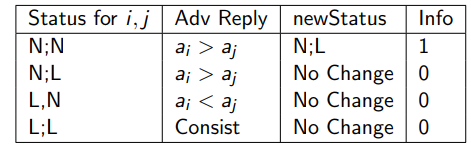
\includegraphics[scale=0.7]{adversary}
\end{center}
\end{document}